\begin{abstract}
Climate change and various anthropogenic factors significantly influence biodiversity and population evolutionary dynamics. To deepen our understanding of the mechanisms driving these disturbances within ecosystems, biologists employ phylogeographic approaches. These methods aim to establish the correlation between the genetic structure of populations and their geographical distribution, considering their current or historical geoclimatic history.

Our laboratory focuses on developing bioinformatics tools to enhance phylogeographic analysis. Recognizing the urgency of the current climate crisis, we are conducting an in-depth analysis of the impact of extreme climatic parameters and environmental factors on Cumacea (crustaceans: Peracarida). Our approach includes a comparative study that validates our phylogeographic models against environmental data from the northern waters of the North Atlantic around Iceland. Concurrently, we are updating a Python package (in beta) to facilitate these complex analyses.
\end{abstract}

\section{Introduction}\label{introduction}
In the greater North Atlantic and subarctic region, the Icelandic region and its adjacent waters are fascinating from an ecological point of view \citep{brix2014iceage, hansen2000north, schnurr2014composition}. The marine region surrounding Iceland contains a great diversity of water bodies of different origins \citep{brix2014iceage} that often meet and overlap \citep{malmberg2003hydrographic, brix2010distribution, meissner2014benthic}. These particular oceanographic and hydrographic conditions shape and influence benthic habitats through depth gradients, water mass indicators, and habitat organization \citep{meissner2014benthic}. Thus, the studies carried out in these regions allow us to deepen our knowledge of the deep-sea ecosystems and biodiversity patterns found in these regions \citep{meissner2018preface}.

Biological and environmental baseline data collected in these regions by the IceAGE project, as well as its predecessors, BIOFAR (Biology of the Faroe Island; \citep{norrevang1994list, gerken1999cumacea}) and BIOICE (Benthic Invertebrates of Icelandic waters; \citep{omarsdottir2013biodiversity}), which explored the biodiversity of the Faroe Islands and Iceland \citep{meissner2018preface}, are invaluable resources. They provide crucial information for understanding two major issues facing present and future generations: the impact of climate change and seabed mining. The North Atlantic region around Iceland has been known for several decades as a critical region for the regulation of global thermohaline circulation \citep{meissner2018preface}. The Greenland, Iceland, and Norwegian (GIN) seas, as well as the high-latitude North Atlantic, play a crucial role in modern deep-sea ventilation. The surface waters of this region are essential source regions for the global deep-sea renewal and are vital for the circulation of thermohaline currents \citep{johannessen1994relationship}. One of the most important changes is the formation of cold, deep water \citep{lohmann1998sea, meehl2007global, winton1997effect}. With the loss of Arctic sea ice, the process of deep-sea formation has slowed, likely impacting flow and chemistry in the region studied during the IceAGE expedition \citep{meissner2018preface}.

There is growing international interest in deep-sea resource extraction, and mining operations are about to begin in some regions \citep{halfar2007danger, mengerink2014call, nath2000environment}. These operations are particularly targeted at mid-ocean ridges and other active geothermal areas. Ridges around Iceland include such areas, such as Reykjanes Ridge, which is home to hydrothermal vent sites. Accurately assessing the extent of damage and loss of ecosystem services caused by mining activities is difficult without robust baseline data \citep{meissner2018preface}.

Crustaceans of the taxon Peracarida Calman, 1904, often constitute a significant portion of macrobenthic communities in Arctic and subarctic waters \citep{brandt1997biodiversity, conlan2008distribution, stransky2010diversity} and may be widely dispersed on the shelf and continental slope of the northern seas \citep{hansen1916crustacea, just1980amphipoda, svavarsson1990distribution, svavarsson1993deep, brandt1995peracarid, brandt1996species}. Most Peracarida are benthic organisms, either infaunal or epifaunal, and they do not have a larval stage \citep{hessler1989behavior, dauvin1996suprabenthic}. In this study, we focus on the peracarid taxon Cumacea Krøyer, 1846. These bottom-dwelling marine benthic crustaceans spend much of their lives buried in or near sediments with a morphology adapted to a lifestyle at the sediment-water interface \citep{uhlir2021adding}. As a result, Cumacea are presumed to have limited dispersal capabilities and are unlikely to drift long distances \citep{rex1981community, wilson1987speciation}.

Unlike benthic invertebrates inhabiting rocky intertidal habitats in the Northwest and Northeast Atlantic \citep{wares2002community, maggs2008evaluating, ilves2010colonization}, very little information is available on the evolutionary history and dynamics of deep-sea benthic invertebrates in the North Atlantic \citep{etter2011phylogeography}. A genetic structure consistent with the expansion of North Atlantic populations farther towards the poles has been detected (e.g., \citep{aarbakke2011discovery}), emphasizing the role and importance of integrating climate change into range expansion studies \citep{jennings2014phylogeographic}. Although studies reveal interesting patterns in the genetic distribution of deep-sea benthic invertebrates (e.g., \citep{havermans2013genetic, wilson1998historical}), a better understanding of the origin and demography of deep Atlantic biota is fundamental to deepening our knowledge of its contemporary connectivity in an evolutionary context and understanding its relationship to ongoing climate change. Continued warming further opens up trans-Arctic lanes \citep{jennings2014phylogeographic}.

\section{Related Works}\label{related-works}
% This section will be filled later.

\section{Materials and Methods}\label{materials-methods}

\subsection{Description of the data}
The study area is located in a northern area of the North Atlantic, including the Icelandic Sea, the Denmark Strait, and the Norwegian Sea. The specimens included in this study were collected during the international IceAGE (Icelandic marine Animals: Genetic and Ecology; Cruise ship M85/3 in 2011; \citep{brix2014iceage, meissner2018preface}) aboard the Meteor RV that explored the deep continental slopes and abyssal waters around Iceland \citep{meissner2018preface}. The data considered in this study from the IceAGE expedition are available via the study of \cite{uhlir2021adding}. The sampling period for the specimens included in this study is from August 30 to September 22, 2011, and they were collected in a depth range of 316-2568 m.

A detailed description of the sampling plan can be found in \cite{brix2014iceage}. Once the benthic sampling gear was brought back on board, its contents were gently poured into the seawater and then evenly distributed over a series of screens of different meshes: 1 mm, 0.5 mm, and 0.3 mm. The material was then washed with seawater on a sieving table before being stored in bulk in 96\% undenatured ethanol, which had been previously cooled. All samples were processed as described in \cite{riehl2014field}, ensuring that the samples remained constantly cooled. The samples were sorted either directly on board or subsequently in the laboratories of the German Centre for Marine Biodiversity Research (DZMB, Senckenberg am Meer, Hamburg, Germany).

Species identification was carried out at the Department of Biological Sciences (University of Bergen, Norway) and DZMB Hamburg using a ZEISS SteREO Discovery V8 or Leica MZ12.5 dissecting microscope. The current authoritative classification followed the World Cumacea Database (\href{http://www.marinespecies.org/cumacea/}{marinespecies.org/cumacea}, \citep{watling2019world}) in the World Register of Marine Species (WoRMS Editorial Board, 2024). In addition, comparative material had been obtained from the Hamburg Centre for Natural History (CeNak) and the University Museum Bergen (ZMBN). The steps of DNA extraction, PCR amplification and sequencing, as well as the extracted and aligned DNA sequences, are available in the article by \cite{uhlir2021adding}.

\subsection{Data pre-processing}
We considered data from the IceAGE project as well as data from the BOLD Systems database, both of which are available via the article by \cite{uhlir2021adding}. Given the large range of attributes from these databases, we made a succinct selection of the number of attributes and samples across them. Thus, we omitted attributes that were not relevant in the context of this study, that were completely or nearly invariable (non-numerical data) as well as those that had abundant missing data (> 95\%). Although the BOLD Systems database contains data on DNA sequences and sample sequencing from the PASCAL (Physical feedbacks of Arctic PBL, Sea ice, Cloud and Aerosol; Cruise ship PS106/1 in 2017; \citep{macke2017physical}), as well as those of the IceAGE expedition, we decided not to include data from the PASCALE project in our analyses. This was because some of their attributes differed or were missing from those in the IceAGE database. We therefore included 62 of the 81 datasets from BOLD Systems in our analysis. Therefore, we considered only 62 of the 495 datasets from the IceAGE project.

Subsequently, we calculated the variance for each of the selected numeric attributes in order to eliminate those with zero or low variance (cut-off ≥ 0.1):

\begin{equation}
S^2 = \frac{\sum_{i=1}^{n} (x_i - \bar{x})^2}{n-1}
\end{equation}

where \( S^2 \) is the variance of the sample, \( x_i \) represents each value in the data set, \( \bar{x} \) the average of all values in the data set, and \( n \) the number of values in the data set.

Of the previously selected numerical attributes, only salinity was removed (\( S^2 = 0.02146629 \)). This selection of attributes and data resulted in a data table containing 62 rows (\( n=62 \)) and 18 columns (number of attributes). Figures \ref{fig:fig1a} and \ref{fig:fig1b} in the appendix were made from Python 3.11.

\begin{figure}[]
    \centering
    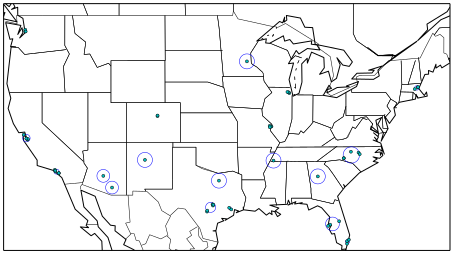
\includegraphics[width=0.7\textwidth]{figure1.png}
    \caption{Geographical coordinates at the beginning of the collection of each sample. \label{fig:fig1a}}
\end{figure}

\begin{figure}[]
    \centering
    \includegraphics[width=0.7\textwidth]{figure2.png}
    \caption{Geographical coordinates at the end of the collection of each sample. \label{fig:fig1b}}
\end{figure}

From the IceAGE database, 14 attributes were selected. These consist of the geographical coordinates such as longitude (decimal) and latitude (decimal) taken at the beginning (see Figure \ref{fig:fig1a} and \ref{fig:fig1b}) and at the end of the collection of each sample. The increase in latitude, in particular, has been highlighted by several studies as being linked to the loss of marine biodiversity on a global scale \citep{rex1993global, lambshead2000latitudinal, gage2004diversity}. These geographic data are divided into five sectors across the seas around Iceland: the Denmark Strait (\( n=28 \)), the Iceland Basin (\( n=15 \)), the Irminger Basin (\( n=12 \)), the Norwegian Sea (\( n=4 \)) and the Norwegian Basin (\( n=3 \)). For the environmental attributes in this database, we included the depth (m) at the beginning and end of sampling (see Figure \ref{fig:fig1c}) as well as the temperature (\( \degree C \)) (see Figure \ref{fig:fig1d}) and oxygen concentration (mg/L) (see Figure \ref{fig:fig1e}) of the water depending on the depth at which the specimens were sampled. These properties of water bodies are drivers of deep-sea biodiversity and biogeography with oxygen being a limiting factor for living organisms \citep{keeling2010ocean}. In addition to these contributions, the increase in depth \citep{rex2006global, roberts2009cold, costello2017marine} as well as the decrease in water temperature at depth \citep{lambshead2000latitudinal} are also factors in the loss of marine biodiversity on a global scale. Meteorological parameters such as speed (m/s) (see Figure \ref{fig:fig1f}) and wind direction at the beginning and end of sampling were also included in our data given the contribution of wind to the restructuring of the benthic ecosystem through water transport \citep{saeedi2022environmental, waga2020recent}. The wind direction at the start of sampling consists of six orientations: South-West (\( n=22 \)), South (\( n=15 \)), North-East (\( n=9 \)), South-South-East (\( n=9 \)), North-West (\( n=5 \)) and East (\( n=2 \)); while the one at the end of the sampling is made up of seven orientations: South (\( n=15 \)), South-West (\( n=15 \)), North-East (\( n=9 \)), West-South-West (\( n=7 \)), South-East (\( n=6 \)), North-North-West (\( n=5 \)), South-South-East (\( n=3 \)) and East (\( n=2 \)). In addition, we have included the sedimentary characteristics of the sampling sites as factors influencing the distribution of Cumacea \citep{uhlir2021adding} and which, for the purposes of this study, fall into six categories: mud (\( n=30 \)), sandy mud (\( n=15 \)), sand (\( n=9 \)), forams (\( n=3 \)), muddy sand (\( n=3 \)) and gravel (\( n=2 \)).

\begin{figure}[]
    \centering
    \includegraphics[width=0.7\textwidth]{figure3.avif}
    \caption{Depth at the beginning and end of sampling. \label{fig:fig1c}}
\end{figure}

\begin{figure}[]
    \centering
    \includegraphics[width=0.7\textwidth]{figure4.png}
    \caption{Temperature (\( \degree C \)) of the water at sampling depth. \label{fig:fig1d}}
\end{figure}

\begin{figure}[]
    \centering
    \includegraphics[width=0.7\textwidth]{figure5.webp}
    \caption{Oxygen concentration (mg/L) of the water at sampling depth. \label{fig:fig1e}}
\end{figure}

\begin{figure}[]
    \centering
    \includegraphics[width=0.7\textwidth]{figure6.png}
    \caption{Wind speed (m/s) at the beginning and end of sampling. \label{fig:fig1f}}
\end{figure}

In the BOLD Systems database, taxonomic ranks such as family, genus, and species of the sampled Cumacea were included in our data. These are composed of seven families of Cumacea: Diastylidae (\( n=21 \)), Lampropidae (\( n=13 \)), Leuconidae (\( n=12 \)), Nannastacidae (\( n=7 \)), Bodotriidae (\( n=4 \)), Ceratocumatidae (\( n=3 \)) and Pseudocumatidae (\( n=2 \)). A total of 21 species of Cumacea are found in our sample (see Figure \ref{fig:fig2}).

\begin{figure}[]
    \centering
    \includegraphics[width=0.7\textwidth]{figure7.webp}
    \caption{Taxonomic distribution of sampled Cumacea species. \label{fig:fig2}}
\end{figure}

The habitat and water mass of the sampling points are the only attributes that were taken directly via Table 1 of \cite{uhlir2021adding}. Thus, the definitions of water bodies described by \cite{hansen2000north}, \cite{brix2010distribution} and \cite{ostmann2014marine} were used as a reference for the GIN seas around Iceland: Arctic Polar Water (APW, \( n=15 \)), Iceland Sea Overflow Water (ISOW, \( n=15 \)), North Atlantic Water (NAW, \( n=9 \)), Arctic Polar Water/Norwegian Sea Arctic Intermediate Water (APW/NSAIW, \( n=7 \)), warm Norwegian Sea Deep Water (NSDWw, \( n=8 \)), Labrador Sea Water (LSW, \( n=3 \)), cold Norwegian Sea Deep Water (NSDWc, \( n=3 \)) and Norwegian Sea Arctic Intermediate Water (NSAIW, \( n=2 \)). In terms of habitat, we considered the three categories used in \cite{uhlir2021adding}: deep sea (\( n=38 \)), shelf (\( n=15 \)) and slope (\( n=9 \)).

The aligned DNA sequence of the mitochondrial 16S rRNA gene region of each of the samples will also be included in our analyses. Thus, we consider 62 of the 306 aligned DNA sequences that were used for phylogenetic analyses of \cite{uhlir2021adding}. Since some of the specimens in our sample have their DNA sequence aligned duplicated, or even quadrupled with a difference of one to two nucleotides, we consider the longest aligned DNA sequence for each of the specimens.

\section{Conclusion}\label{conclusion}

The objective of this study is to perform an in-depth analysis of the influence of extreme climatic variables and environmental characteristics around Iceland on Cumacea (crustaceans: Peracarida) based on phylogeographic analysis. To date, we have selected relevant attributes for our study based on data from the IceAGE project, BOLD Systems, and the study by \cite{uhlir2021adding} and eliminated those that were not relevant to this study as well as those that had low variance (salinity, \( S^2 = 0.02146629 \)) or abundant missing data (>95\%). Thus, the first part consisted mainly of literature review, data collection, data pre-processing, and data analysis.

For the upcoming fall semester, we are planning several crucial steps. First, we'll cluster our data to better understand climate data partitioning. Next, we'll update our Python package (in beta), dedicated to simplifying phylogeographic analyses. We also plan to conduct a thorough genetic analysis to examine the genetic diversity of our samples. In addition, we will analyze the cross-integration of climate and genetic data to better understand the interactions between the environment and the genetics of the populations studied. Finally, we plan to submit a scientific paper before the end of November.